%
% teil1.tex -- Beispiel-File für das Paper
%
% (c) 2020 Prof Dr Andreas Müller, Hochschule Rapperswil
%
%
% teil2.tex -- Beispiel-File für teil2 
%
% (c) 2020 Prof Dr Andreas Müller, Hochschule Rapperswil
%
\documentclass[11pt,a4paper]{article}

\usepackage[utf8]{inputenc}
\usepackage{graphicx}
\usepackage{german}


\pagestyle{myheadings}
\pagenumbering{arabic}

\setlength{\textwidth}{15cm}
\setlength{\textheight}{22cm}
\setlength{\topmargin}{-1cm}
\setlength{\oddsidemargin}{0,5cm}
\setlength{\parindent}{0cm}
\setlength{\headsep}{1,5cm}


\begin{titlepage} % Titelseite einrichten
\title{\bf {Beispieldatei}}

\author{\vspace{2cm}
  Autor}

\date{\vspace{3cm} % Datumsfeld einrichten
      letzte Aktualisierung: \today}

\thispagestyle{empty} % Die Titelseite soll keine Seitenzahl bekommen...[1]
\end{titlepage}



\begin{document}



\section{Kalman Filter}
\subsection{Geschichte}
Der Kalman Filter wurde 1960 von Rudolf Emil Kalman entdeckt und direkt von der NASA für die Appollo Mission benutzt. Der Filter kommt mit wenig Rechenleistung aus und war somit dafür geeignet die Rakete bei der Navigation zu unterstützen. Der Filter schätzt den Zustand eines Systems anhand von Messungen und kann den nächsten Zustand erraten. Typische Anwendungen des Kalman-Filters sind die Glättung von verrauschten Daten und die Schätzung von Parametern und kommt heutzutage in jedem Satellit, Navigationssystem, Smartphones und Videospielen vor.

\subsection{Wahrscheinlichkeit}
Der Kalman Filter versucht nichts anderes, als ein geeigneter Wert zwischen zwei Normalverteilungen zu schätzen. Die eine Kurve zeigt die errechnete Vorhersage des Zustands, bzw. deren Normal- Gauss-Verteilung. Die andere Kurve zeigt die verrauschte Messung des nächsten Zustand, bzw. deren Normal-Verteilung. Wie man in am Beispiel dieser zwei Gauss-Verteilungen sehen kann, ist sowohl der geschätzte Zustand als auch der gemessene Zustand nicht am selben Punkt. 

\begin{figure}[h]
 \begin{center}
 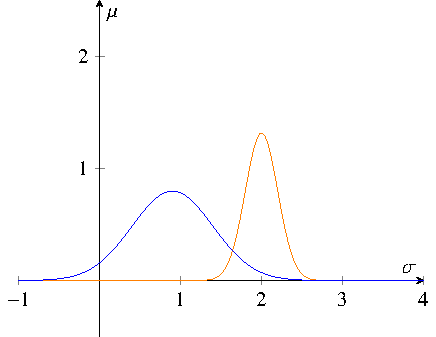
\includegraphics[width=5cm]{Gausskurve2}
 \caption{Zwei Gauss-Verteilungen}
 \end{center}
\end{figure}
Um eine genauere Schätzung des Zustandes zu machen wird nun ein Wert zwischen den beiden Verteilungen gesucht. An diesem Punkt wird nun eine Eigenschaft ausgenutzt. Durch das Multiplizieren zweier Normal-Verteilungen entsteht eine neue Normal-Verteilung. 

Wir haben eine Normalverteilung der Vorhersage:

\begin{equation}
{y_1}(x;{\mu_1},{\sigma_1})=\frac{1}{\sqrt{2\pi\sigma_1^2}}*e^{-\frac{(x-{\mu_1})^2}{2{\sigma_1}^2}}
\end{equation} 
und für die Messung:

\begin{equation}
{y_2}(x;{\mu_2},{\sigma_2})=\frac{1}{\sqrt{2\pi\sigma_2^2}}*e^{-\frac{(x-{\mu_2})^2}{2{\sigma_2}^2}}.
\end{equation} 

Diesen werden nun Multipliziert und durch deren Fläche geteilt um sie wieder zu Normieren:
\begin{equation}
{y_f}(x;{\mu_f},{\sigma_f})=\frac{ \frac{1}{\sqrt{2\pi\sigma_1^2}}*e^{-\frac{(x-{\mu_1})^2}{2{\sigma_1}^2}} *\frac{1}{\sqrt{2\pi\sigma_2^2}}*e^{-\frac{(x-{\mu_2})^2}{2{\sigma_2}^2}}}{\int {y_1}*{y_2}\,}
\end{equation} 

Dadurch gleicht sich die neue Kurve den anderen an. Interessant daran ist, dass die fusionierte Kurve sich der genauere Normal-Verteilung anpasst. ist ${\sigma_2}$ klein und ${\sigma_1}$ gross, so wird sich die fusionierte Kurve näher an ${y_2}(x;{\mu_2},{\sigma_2})$ begeben. 

 \begin{figure}[h]
 \begin{center}
 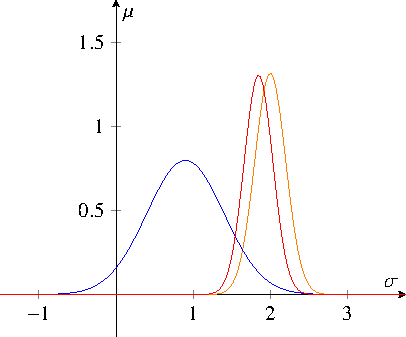
\includegraphics[width=5cm]{Gausskurve3}
 \caption{Produkt der Gauss-Verteilungen}
 \end{center}
\end{figure}
Was in 2 Dimensionen erklärt wurde, funktioniert auch in mehreren Dimensionen. Dieses Prinzip mach sich der Kalman Filter zu nutze, und wird von uns für die Erdbeben Berechnung genutzt. 

\subsection{Anwendungsgrenzen}
Nicht lineare Systeme %Noch nicht Fertig


\section{Aufbau}
Um ein Erdbeben kenntlich zumachen werden in der Regel Seismographen mit vielen Sensoren verwendet. 
Der Seismograph besteht im Grunde aus einer Federgelagerten Masse. Wirkt eine Bodenerregung auf das Gerat ein, bleibt die gekoppelte Masse in der Regel stehen und das Gehäuse schwingt mit.Relativbewegung des Bodens kann damit als Längenänderung im Zeitverlauf gemessen werden. In modernen Seismographen wird die Bodenbewegung in alle Richtungen gemessen, sowohl Horizontal als auch Vertikal. 
Wir konstruieren uns eine einfachere Version eines Seismographen, welcher rein Mechanisch funktioniert. Zudem kann er nur in eine Dimension Messwerte aufnehmen. Würde das System ausgebaut werden, um alle Horizontalbewegungen aufzunehmen, würde der Verwendung des Kalman Filters zu kompliziert werden. Für zwei Dimensionen (x,y) würde der Pythagoras für das System benötigt werden. Da sich der Pythagoras bekanntlich nicht linear verhält, kann kein linearer Kalman Filter implementiert werden. Da der Kalman Filter besonders effektiv und einfach für lineare Abläufe geeignet ist, würde eine Zweidimensionale Betrachtung den Rahmen dieser Arbeit sprengen. 
\begin{figure}[h]
 \begin{center}
 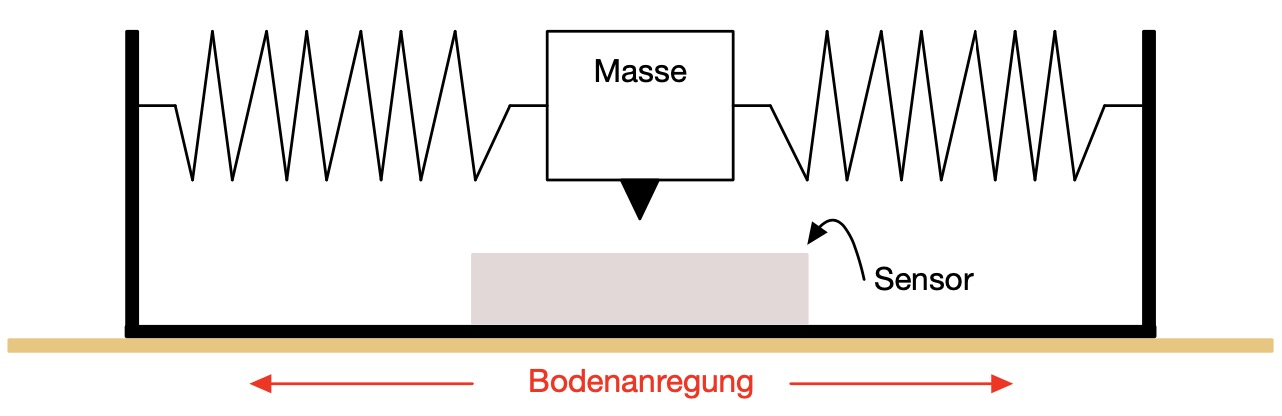
\includegraphics[width=10cm]{Apperatur}
 \caption{System}
 \end{center}
\end{figure}


\subsection{Optionen}
Wollte man einen 2D Seismographen aufbauen, ohne den Pythagroas zu verwenden, kann dies mit der Annahme, das die Feder sehr lang sind erfolgen. Da sich bei langen Federn die Auslenkungen verkleiner...!!Noch nicht fertig!

\section{Systemgleichung}
Da der Kalman Filter zum schätzen des nächsten Zustand verwendet werden kann, wird eine Gleichung welche das System beschreibt. Im Fall unseres Seismographen kann der die Differentialgleichung zweiter Ordnung einer Erzwungene Schwingung am harmonischen Oszillator verwendet werden. Diese lautet:
\begin{equation}
m* \ddot x + 2k *\dot x + D*x = f
\end{equation}
mit den Konstanten m = Masse, k = Dämpfungskonstante und D  = Federkonstante.
Um diese nun die Systemmatrix umzuwandeln, wird aus der Differentialgleichung zweiter Ordnung durch eine Substitution eine DGL erster Ordnung:

\begin{equation}
{x_1}=x, 
{x_2}=\dot x, 
{x_3}=\ddot x \mid Substitution
\end{equation}


\begin{equation}
m* {x_3}+ 2k*{x_2} + D*{x_1} = f \mid DGL  \:1. Ordnung
\end{equation} 

\begin{equation}
{x_3}=-\frac{D}{m} *{x_1} -\frac{2*k}{m} *{x_2} + \frac{f} {m}  \mid  Nach  \: {x_3} 
\end{equation} 

Um die lineare Differentialgleichung in in den Kalman Filter zu Implementieren, muss dieses als Vektor-Gleichung umgewandelt werden. Dafür wird die Gleichung abgeleitet in die Zustände aufgeteilt. Die für uns relevanten Zustände sind die Position der Masse, die Geschwindigkeit der Masse und äussere Beschleunigung des ganzen System. Dabei muss unterschieden werden. um welche Beschleunigung es sich handelt. Das System beinhaltet sowohl eine Beschleunigung der Masse bzw. Feder (innere Beschleunigung), als auch eine Beschleunigung der ganzen Apparatur (äusseren Beschleunigung). In unserem Fall wird die äussere Beschleunigung gesucht, da diese der Erdbeben Anregung gleich kommt. 
\begin{equation}
\frac{d}{dt} \left(\begin{array}{c} {x_1} \\ {x_2}  \end{array}\right) = \left(
 \begin{array}{ccc} 	
0 & 1& 0 \\ 
- \frac{D}{m} &-\frac{2*k}{m} & \frac{1} {m}\\
\end{array}\right)  \left(\begin{array}{c} {x_1} \\ {x_2} \\ {x_3} \end{array}\right).
\end{equation}

Durch die Rücksubstituion ergibt sich:
\begin{equation}
\frac{d}{dt} \left(\begin{array}{c} x(t) \\ v(t) \end{array}\right) = \left(
 \begin{array}{ccc} 	
0 & 1& 0 \\ 
- \frac{D}{m} &-\frac{2*k}{m} & \frac{1} {m}\\
\end{array}\right)  \left(\begin{array}{c} x(t)\\ v(t)\\ f(t) \end{array}\right).
\end{equation}


Da die Kraft unbekannt ist, wird die letzte Teile mit Nullen bestückt, denn genau diese Werte wollen wir. 

\section{Kalman Filter}
Um den Kalman Filter zu starten müssen gewisse Bedingungen definiert werden. In diesem Abschnitt werden die einzelnen Parameter/Matrizen erläutert und Erklärt, für was sie nützlich sind. 
\subsection{Anfangsbedingungen}
\subsubsection*{Anfangszustand x}
Der Filter muss wissen wie das System startet. in unserem Fall is es die Ruhelage, die Masse bewegt sich nicht. Zudem erfährt die Apparatur keine äussere Kraft. 

\begin{equation}
{x_0 }= \left( \begin{array}{c} 0\\ 0\\ 0\end{array}\right)
\end{equation} 

\subsubsection*{Anfangsfehler / Kovarianzmatrix}
Da auch der Anfangszustand fehlerhaft sein kann, wird für den Filter eine Kovarianzmatrix eingeführt. In unserem Fall ist der Anfangszustand gut Bekannt und die Matrix kann mit Nullen bestückt werden. Somit ergibt sich für die Kovarianzmatrix
\begin{equation}
{P_0 }=
\left(
\begin{array}{ccc} 	
0 & 0 &0 \\ 
0 &0 & 0 \\ 
0 & 0 &0 \\
\end{array}
\right).
\end{equation}
Wäre auch der Initialzustand fehlerhaft, könnte über die Diagonale die Kovarianz angegeben werden.
Diese Matrix geht am häufigsten durch den Filter. Sie wird für die Vorhersage und für den Korrekturschritt verwendet und verändert. Für einen gut bekannten Zustandsvektor können kleine Werte eingesetzt werden, für ungenaue Anfangsbedingungen sollten grosse Werte (1 Million) verwendet werden. Bei grossen Werten wird dem Filter die Möglichkeit gegeben, sich schnell einzupendeln. 

\subsubsection*{Dynamikmatrix A}
Die Dynamikmatrix bildet den Kern des Filters. Diese wurde weiter oben Bereits beschrieben. Dabei wollen wird die äussere Kraft des Systems ermitteln.
Da nichts über die äussere Kraft bekannt ist, können wir annehmen das deren Ableitung 0 ist.
Die System Vektor-Gleichung lautet daher:


\begin{equation}
A = \left(
 \begin{array}{ccc} 	
0 & 1& 0 \\
- \frac{D}{m} &-\frac{2*k}{m} & \frac{1} {m}\\
0 & 0& 0\\ 
\end{array}\right)  
\end{equation} 

\subsubsection*{Prozessrauschkovarianzmatrix Q}
Die Prozessrauschmatrix teilt dem Filter mit, wie der Systemzustand vom aktuellen zum nächsten Schritt gehen kann. Dabei wird wieder ein Fehler/Rauschen dazu gerechnet. Bei unserem Modell könnte das Beispielsweise ein Windstoss an die Masse sein. für uns wäre dies:
\begin{equation}
Q = \left(
 \begin{array}{ccc} 	
{\sigma_x }^2& 0& 0 \\ 
0 & {\sigma_v }^2& 0\\ 
0 & 0& {\sigma_f }^2\\
\end{array}\right)  
\end{equation} 

Die Standabweichungen müssten Statistisch ermittelt werden, da der Fehler nicht vom Sensor kommt und somit nicht vom Hersteller gegeben ist. 

\subsubsection*{Messmatrix H}
Die Messmatrix gibt an, welcher Parameter gemessen werden soll. in unsrem Fall ist es nur die Position der Masse. 
\begin{equation}
H= ( \: \: 1 \: \:0 \: \:0 \: \:)
\end{equation} 

\subsubsection*{Messrauschkovarianz R}
Die Messrauschkovarianzmatrix beinhaltet, wie der Name es schon sagt, das Rauschen der Messesensoren. In unserem Fall wird nur die Position der Masse gemessen. Da wir keine anderen Sensoren haben, welche etwas messen kürzt sich diese einfach zu
\begin{equation}
R= ({\sigma_x }^2)\: \: ab.
\end{equation} 
Diese Messrauchen wird meistens vom Sensorhersteller angegeben. Für unsere Theoretische Apparatur wird hier ein kleiner Fehler eingesetzt.

\subsection{Fiter Algorithmus}
Nachdem alle Parameter aufgestellt sind, wird der Filter initialisiert und Versucht nun den Zustand der Feder Vorherzusagen, die Messung zu Präzisieren und laufend zu Aktualisieren. Dank der fortlaufender Messung Bleibt die Schätzung des Filters immer relativ genau. In diesem Abschnitt werden alle Rechenschritte, welche über die ganze Zeitdauer läuft und stetig aktualisiert wird, aufgezeigt und Aktualisiert.


\subsubsection*{Vorhersage}
Im Filterschritt Vorhersage wird der nächste Zustand anhand des Anfangszustand und der Systemmatrix berechnet. Dies funktioniert ganz Trivial mit dem Rechenschritt:
\begin{equation}
{x_{t+1}}=A*{x_t}.
\end{equation} 


Die Kovarianz $P_{pred}$ wird im nächsten Schritt ebenfalls neu berechnet, da die Unsicherheit im $Vorhersage$ grösser wird als im Aktuellen. Da wir ein Mehrdimensionales System haben kommt noch die Messunsicherheit $Q$ dazu, so dass die Unsicherheit des Anfangsfehlers $P$ immer grösser wird. Dies funktioniert durch multiplizieren der Systemmatrix, deren Ableitung und mit dem aktualisierten Anfangsfehler. Dazu wird noch die Messunsicherheit addiert, somit entsteht die Gleichung


\begin{equation}
{P_{pred}}=A*P*A`+Q.
\end{equation}

wird dieser Vorgang wiederholt, schaut der Filter wie genau die letzte Anpassung von $P$ zur Messung stimmt. Ist der Unterschied klein, wird die Kovarianz $P$ kleiner gewählt, ist der Unterschied gross, wird der Filter auch die Kovarianz grösser wählen. Er passt sich selber an und korrigiert sich bei grosser Abweichung.

\subsubsection*{Messen}
Der Sensor wurde noch nicht benutz, doch genau der liefert Werte für den Filter. Die aktuellen Messwerte $Z$ werden die Innovation $w$ mit dem Zustandsvektor $x$ und der Messmatrix $H$ zusammengerechnet.
Hier bei wird lediglich die Messung mit dem Fehler behaftet, und die Messmatrix $H$ 
\begin{equation}
w=Z-(H*x)
\end{equation}
Im nächsten Schritt wir analysiert, mit welcher Kovarianz weiter gerechnet wird. 

\subsubsection*{Korrigieren}
Udpdate
\section{Anfügen der Schwingung}

Ein Erdbeben breitet sich im Boden wellenartig aus und bringt Objekte, wie zum Beispiel ein Gebäude, in Schwingung.
Diese Schwingungen pflanzen sich im Gebäude mit gleicher Amplitude, Geschwindigkeit und Beschleunigung in horizontaler und vertikaler Bewegung fort.
Wir möchten herauszufinden, wie gross die Massenbeschleunigung infolge eines Erdbeben ist.
Mit Hilfe von fiktiven Sensoren, die eine Ortsveränderung des Gebäude messen, können wir mit Anwendung von Matrizen und dem Kalman-Filter die Beschleunigung berechnen.

\begin{equation}
\int_a^b x^2\, dx
=
\left[ \frac13 x^3 \right]_a^b
=
\frac{b^3-a^3}3.
\label{erdbeben:equation1}
\end{equation}

\section{Erreger-Schwingung}
Wir möchten mit einer gedämpften harmonischen Schwingung ein einfaches Erdbeben simulieren, die im Kalman Filter eingespeist wird.
Die Gleichung lautet

\begin{equation}
x(t)=A*e^{t/2}*sin(t).
\end{equation}

Mit dieser Schwingung können wir ein einachsiger Seismograph simulieren, der eine Ortsverschiebung auf der x-Achse durchführt.
Die Dämpfung der Schwingung ist relevant, da das System beim Schwingungsvorgang durch die Federkonstante und der Reibung, Energie verliert.

Die Ergebnisse dieser Schwingung setzen wir in die Messmatrix ein und können den Kalman-Filter starten.





\end{document}
